\documentclass{beamer}

\usepackage[ngerman]{babel}
\usepackage[utf8]{inputenc}
\usepackage[T1]{fontenc}
\usepackage{color}
\usepackage{lmodern}
%\usepackage{enumitem}
%	\setitemize{label=\usebeamerfont*{itemize item}%
%	\usebeamercolor[fg]{itemize item}
%	\usebeamertemplate{itemize item}}
\usepackage{amsmath}
\usepackage{array,arydshln} % dashed hlines
\usepackage{CJKutf8}
\usepackage{bxcjkjatype}
\usepackage{tikz}
	\newcommand{\adjustTikzSize}[0]{\Large}
	\newcommand{\tikzScale}[0]{0.75}
\usepackage{amssymb}
\usepackage{graphicx}
	\graphicspath{{img/}}
\usepackage{nicefrac}
\usepackage{csquotes}
\usetheme{Frankfurt}
	\usefonttheme{structurebold}
	\usecolortheme{rose}
\newtheorem*{bem}{Bemerkung}
\newtheorem*{bsp}{Beispiel}
\usepackage{parskip}
%absolute figure positioning
\usepackage[absolute,overlay]{textpos}
  \setlength{\TPHorizModule}{1mm}
  \setlength{\TPVertModule}{1mm}
\usepackage[backend=bibtex, style=authoryear]{biblatex} 
\addbibresource{literature.bib}

\definecolor{cgray}{gray}{0.35}
\newcommand{\scite}[1]{ {\scriptsize \textcolor{cgray}{(\cite{#1})}} }


  
\defbibenvironment{bibliography}
{\list{}
{\setlength{\itemsep}{6px}%
\setlength{\parsep}{\bibparsep}}}
{\endlist}
{\item \scriptsize}

\definecolor{mygrey}{RGB}{80,80,80}

\setbeamertemplate{headline}
{%
\hfill
\textbf{\insertsection} \
\insertsubsection \
\insertframenumber / \inserttotalframenumber
}
\setbeamertemplate{navigation symbols}{}

\title{Integrating Probabilistic and Database Models for Rapidly Building Customized Machine Learning Applications\vspace*{.4em}}
%Integration von probablistischen und Datenbankmodellen zur schnellen Entwicklung individuell zugeschnittener Machine-Learning-Anwendungen
\author{
\vspace*{-1em}
Frank Rosner
}

\institute{
Martin-Luther-Universität Halle-Wittenberg
}
\date{26. September 2014}

\begin{document}

\frame{\titlepage 
\parbox{0cm}{\tiny 
\vspace{-30pt}\color{mygrey}
\begin{tabbing}
XXXXXXXXXXXXXXXXXXXXXIXXX\=XXXXXXXX\= \kill \\
\>Gutachter:\> Dr. Alexander Hinneburg \\
\>\> Prof. Stefan Brass
\end{tabbing}
}}

\begin{frame}[t]{Motivation}
\vspace*{1.5em}
\begin{itemize}
\item wachsende Datenmassen weltweit
\item Daten als wirtschaftliches Gut\scite{forum2012bigdata}
\end{itemize}

\begin{textblock}{50}(70,70)
	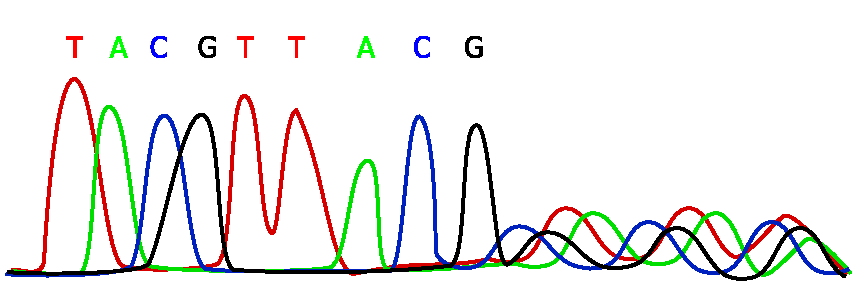
\includegraphics[width=1\linewidth]{electropherogram}
\end{textblock}
\begin{textblock}{25}(10,50)
	
\includegraphics[width=1\linewidth]{binary-file}
\end{textblock}
\begin{textblock}{20}(70,45)
	
\includegraphics[width=1\linewidth]{globe}
\end{textblock}
\begin{textblock}{10}(90,40)
	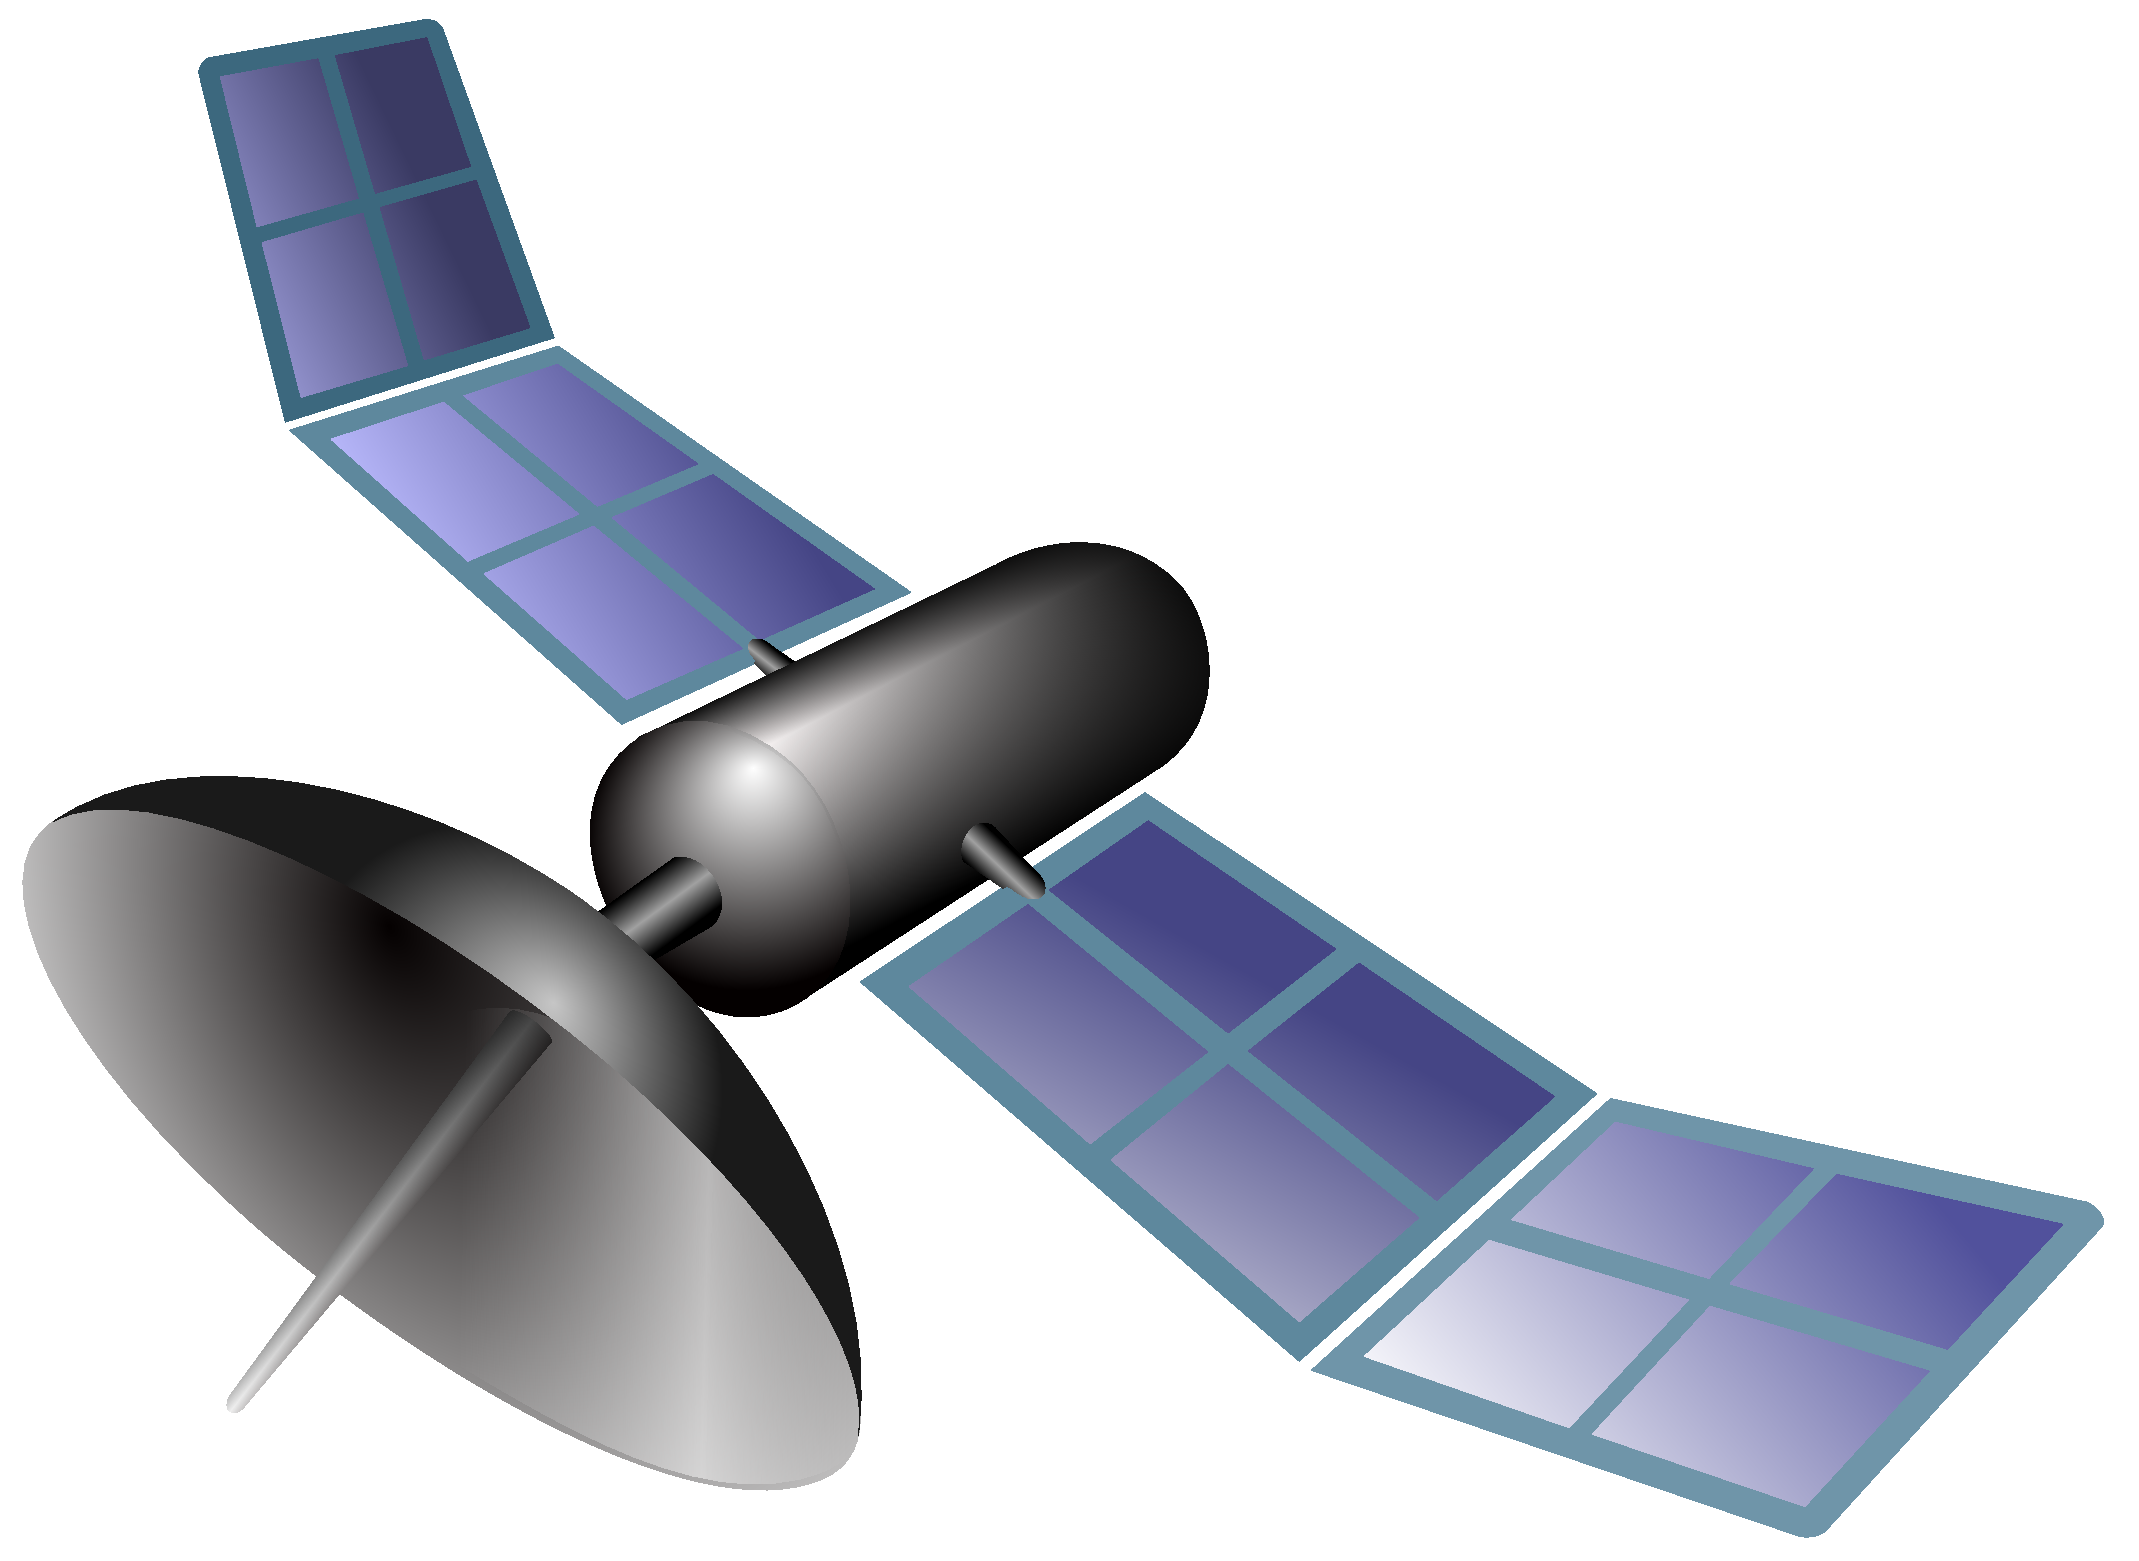
\includegraphics[width=1\linewidth]{satellite}
\end{textblock}
\begin{textblock}{10}(100,50)
	
\includegraphics[width=1\linewidth]{gps}
\end{textblock}
\begin{textblock}{25}(40,60)
	
\includegraphics[width=1\linewidth]{db}
\end{textblock}
\end{frame}

\begin{frame}[t]{Motivation}
\begin{itemize}
\vspace*{1em}
\item \enquote{Data Scientist: Der attraktivste Beruf des 21. Jahrhunderts} \scite{davenport2012data}
	\begin{itemize}
	\item Statistik, Machine-Learning, Mustererkennung, Data Mining
	\item Informatik, effiziente Algorithmen, Datenverwaltung
	\end{itemize}
\end{itemize}

\vspace*{1em}
\textbf{Problem:} Datenflut nicht von Flut an Data Scientists begleitet

\vspace*{3em}
\begin{center}
{\Large Individuell zugeschnittene Analysen}\hspace*{4em}

{\Large ohne Data Scientists?}\hspace*{4em}
\end{center}

\begin{textblock}{30}(93,57)
	
\includegraphics[width=1\linewidth]{scientist}
\end{textblock}
\end{frame}

\begin{frame}
\frametitle{Gliederung}
\tableofcontents
\end{frame}

\section{Problemstellung}
\frame{\frametitle{Gliederung} \tableofcontents[currentsection]}
\begin{frame}{Test}

x
\begin{definition}[Definition]
y
\end{definition}

\begin{bem}[Bemsss]
x
\end{bem}
\end{frame}

\section{Zielstellung}
\frame{\frametitle{Gliederung} \tableofcontents[currentsection]}
\begin{frame}

\end{frame}

\section{Hauptteil}
\frame{\frametitle{Gliederung} \tableofcontents[currentsection]}
\begin{frame}

\end{frame}

\section{Zusammenfassung}
\frame{\frametitle{Gliederung} \tableofcontents[currentsection]}
\begin{frame}

\end{frame}

\section{Ausblick}
\frame{\frametitle{Gliederung} \tableofcontents[currentsection]}
\begin{frame}

\end{frame}

\section{Quellen}
\frame{\frametitle{Gliederung} \tableofcontents[currentsection]}
\begin{frame}
\frametitle{Quellen}
\def\bibfont{\scriptsize}
\printbibliography
\end{frame}

\end{document}